\documentclass[10pt]{article}
\usepackage{parskip}
\usepackage[utf8]{inputenc}
\usepackage[left=2.00cm, right=2.00cm, top=2.00cm, bottom=2.00cm]{geometry}
\usepackage[spanish]{babel}
\usepackage{graphicx,subfig}
\usepackage{fancyhdr}
\usepackage[rightcaption]{sidecap}
\usepackage[font=small,labelfont=bf]{caption}
\usepackage[american]{circuitikz}
\graphicspath{{Imagenes/}}
\usepackage{enumerate} 
\usepackage{multicol}
\usepackage{tabularx}
\usepackage{amssymb}
\usepackage{adjustbox}
\usepackage{amsmath}
\usepackage{cancel}
\begin{document}


\pagestyle{fancy}
\cfoot{}


%Cabeceras
\rhead{Practica 1}
\lhead{ESIMEZ-ICE}

%Portada
\begin{titlepage}
	\newgeometry{
		left=25mm,
		right=25mm,
		top=5mm,
		bottom=30mm,
		headheight = 0 mm
	}

	\begin{figure}[t]
		\subfloat{
\includegraphics[width=0.15\textwidth]{Logo_IPN}}
		\hspace{0.6\textwidth}
		\subfloat{
\includegraphics[width=0.22\textwidth]{LogoEsime}}
	\end{figure}

	\centering
	{\bfseries\Huge Instituto Politécnico Nacional. \par}
	\vspace{1cm}
	{\scshape\Large Ingeniería en Comunicaciones y Electrónica. \par}
	\vspace{0.3cm}
	{\scshape\Large Laboratorio de Circuitos de C.A y C.U .  \par}
	\vspace{1cm}
	{\scshape\Huge Mediciones Mixtas. \par}
	{\itshape\Large Practica 1. \par}
	\vspace{1cm}
	{\Large 3CM7\par}
	\vfill
	{\Large Autor: \par}

	{\Large José Emilio Hernández Huerta. \par}

	\vfill
	{\Large Septiembre 2023. \par}

\end{titlepage}

\tableofcontents
\newpage

\section{Resumen.}
Con un circuito de 6 elementos pasivos, en particular 4 recistores en serie, 2 en paralelo y una fuente de corriente continua,  de cada elemento se calcuaron sus recistencias individuales y equivalente, sus corrientes individuales y sus potencias individuales por 4 metodos diferentes; teorico, practico, simulacion en Multisim y simulacion en Pspice 

\begin{multicols}{2}

\section{Objetivo.}
Calcular las magnitudes de los componentes electronicos, como aprender a simular circuitos en programas profesionales como Multisim y Pspice. Conocer el funcionamiento de la protoboard al igual de como medirlos con un multimetro tomando las medidas optimas para no quemar ningun fusible, recistor o fuente.



\section{Marco teórico.}

\subsection{El multímetro.}
Un multímetro digital, como el LOMVUM T28B, se utiliza para medir voltaje, corriente, resistencia y otras magnitudes eléctricas en circuitos. Tiene una pantalla LCD para mostrar los valores y perillas de selección para elegir la función de medición. Los cables de prueba se conectan al componente o circuito que se va a medir. Puedes medir voltaje en paralelo, corriente en serie y resistencia conectando los cables adecuadamente. Los multímetros avanzados pueden tener funciones adicionales como medición de capacitancia y continuidad. 
	\begin{center}
		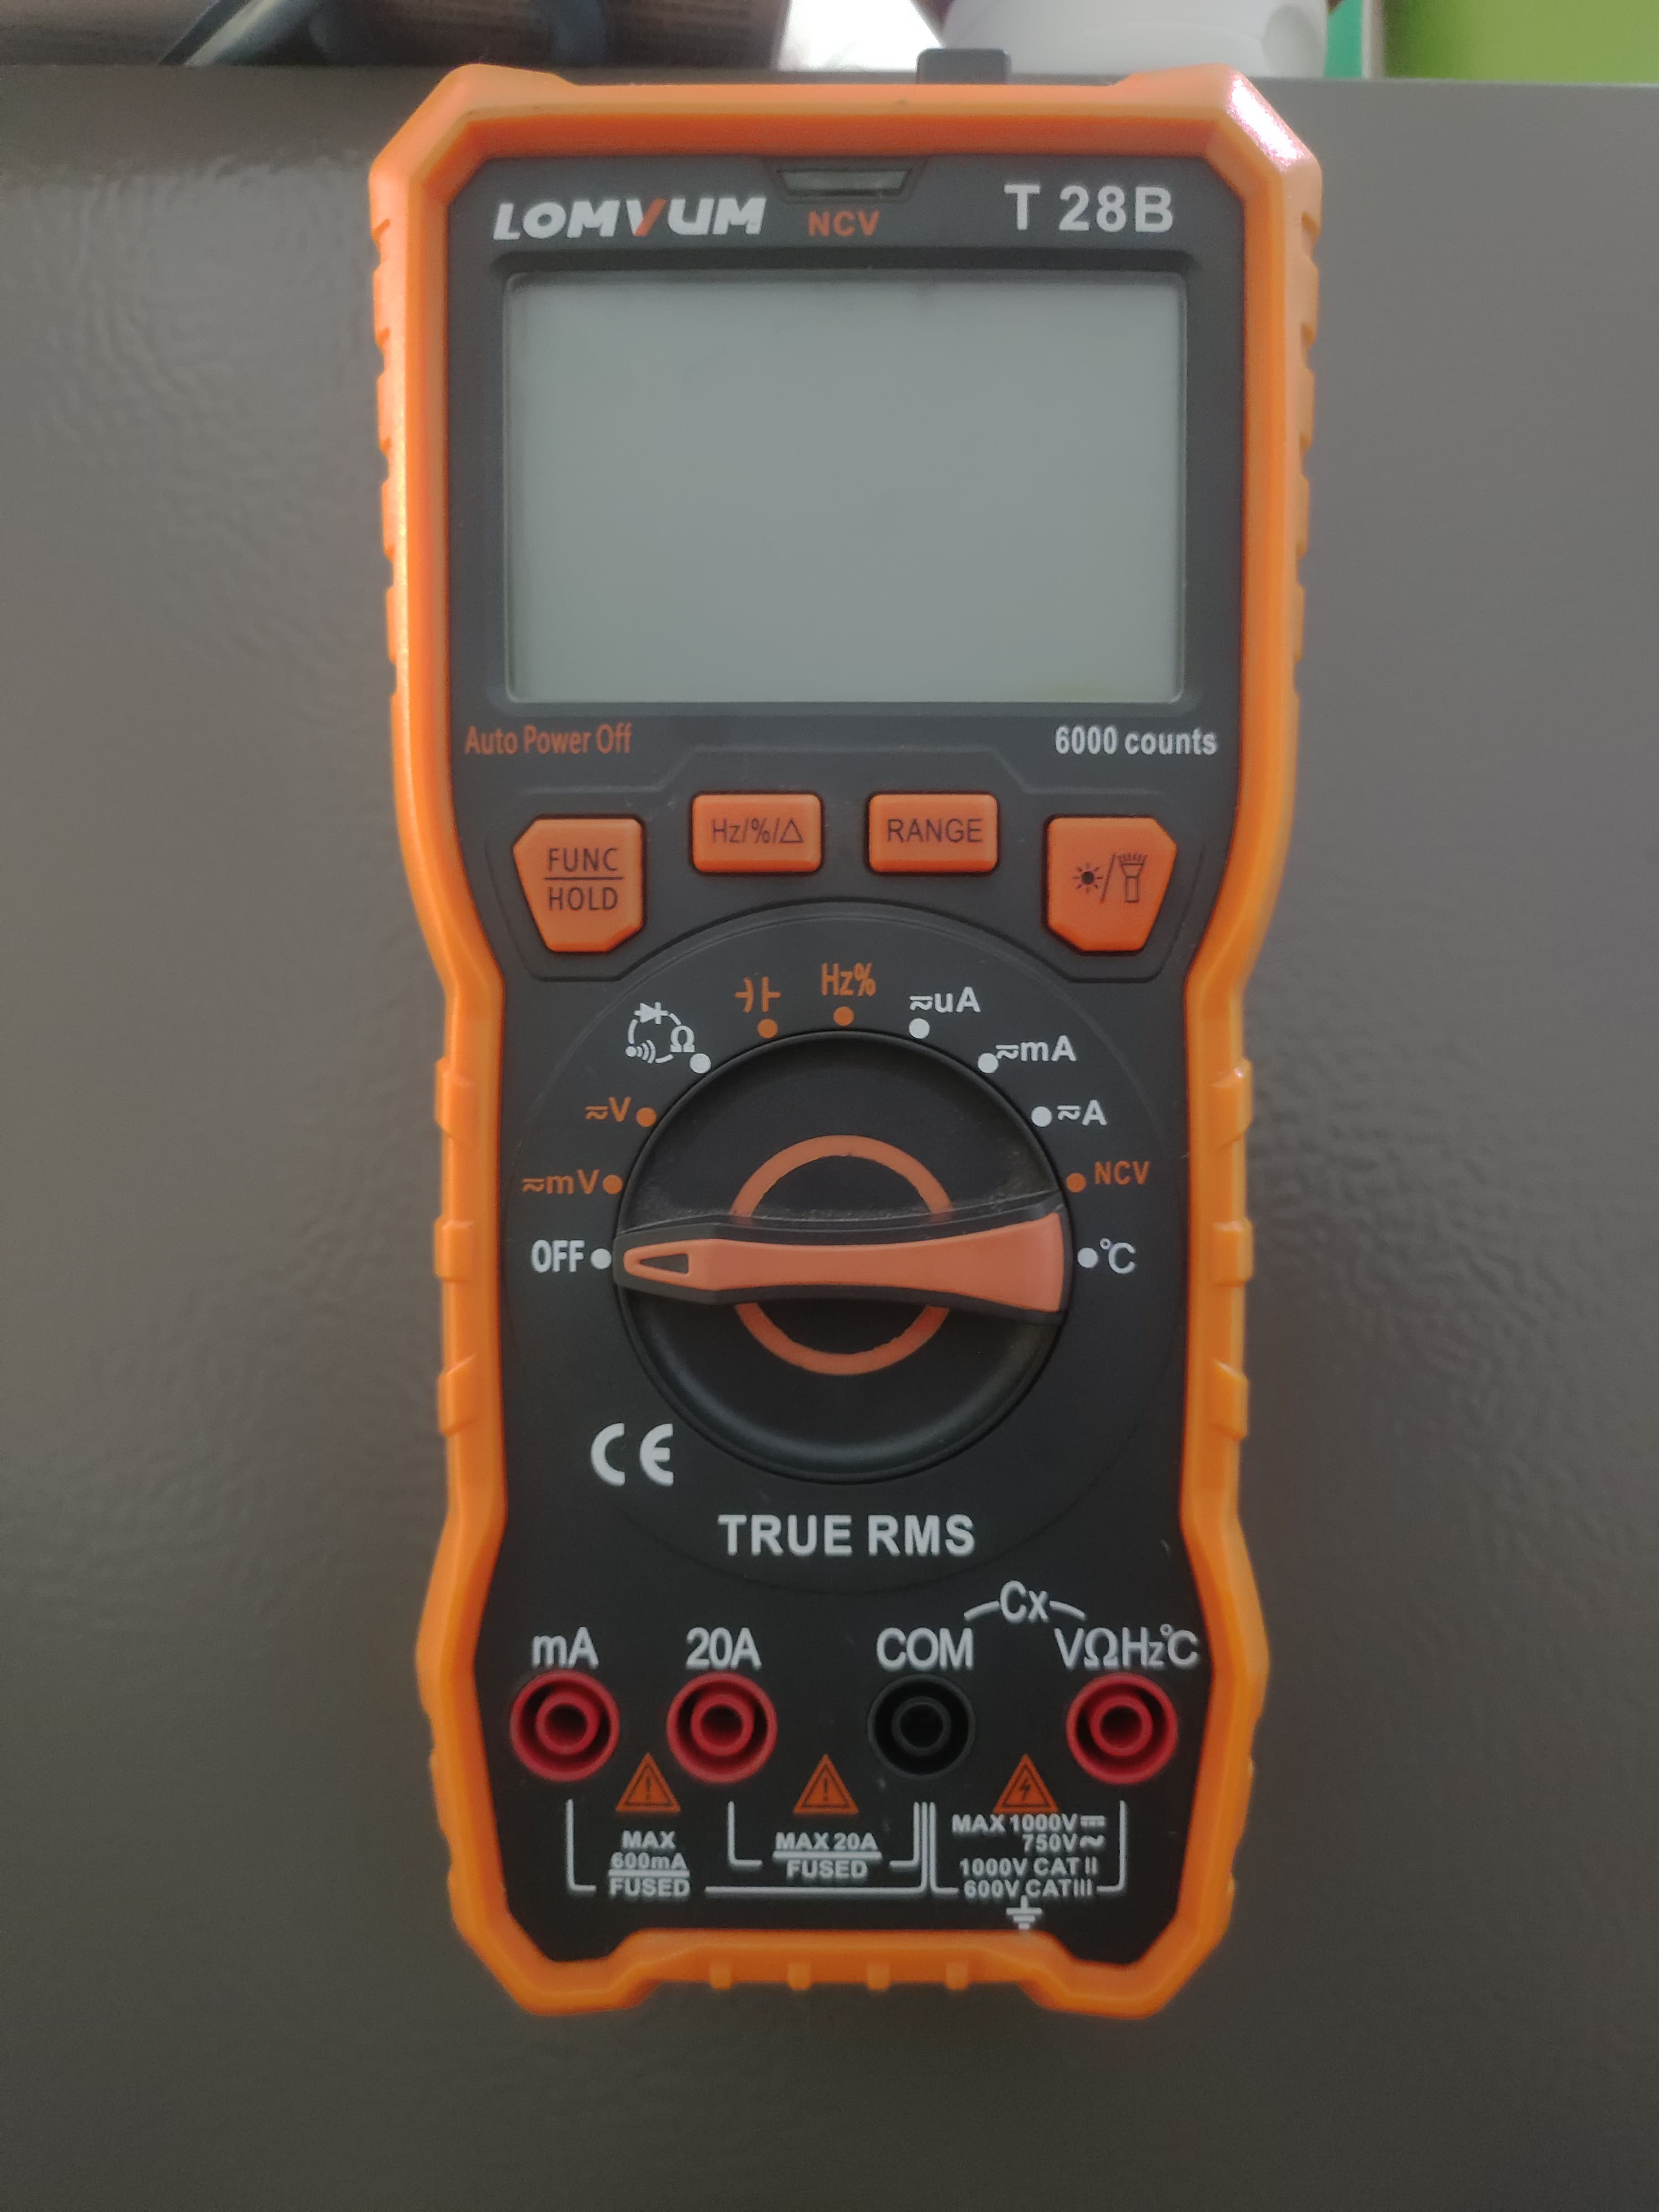
\includegraphics[width=3cm, height=4cm]{Imagenes/Multimetro.jpeg}
		\captionof{figure}{Multimetro}
		
	\end{center}
	
	
		
	
	

\subsection{Fuente regulable.}
Una fuente regulable de corriente continua (CC) es un dispositivo que suministra una corriente constante y ajustable a un circuito o carga. Funciona mediante la conversión de corriente alterna (CA) en CC a través de un transformador y un rectificador, seguido de un circuito de regulación de corriente que permite ajustar la corriente deseada. Estas fuentes son esenciales en laboratorios y aplicaciones electrónicas, permitiendo un suministro preciso y controlado de energía a dispositivos y circuitos. Además, a menudo incluyen protecciones para evitar condiciones peligrosas.
\begin{center}
	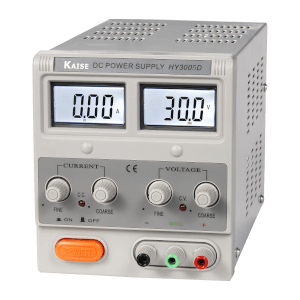
\includegraphics[width=3cm, height=4cm]{Imagenes/fuente.png}
	\captionof{figure}{Fuente de voltaje regulable}
	
\end{center}

\subsection{Protoboard.}
La protoboard consiste en una superficie rectangular con una serie de orificios pequeños distribuidos en filas y columnas. Cada uno de estos orificios está conectado eléctricamente con otros orificios en su misma fila o columna. Las filas y columnas están etiquetadas con números y letras, lo que facilita la organización y la conexión de los componentes.

Lo que hace que la protoboard sea tan útil es que permite conectar componentes electrónicos, como resistencias, LEDs, transistores y otros, simplemente insertando sus patas en los orificios correspondientes. Cuando dos componentes comparten un orificio o están conectados a través de un cable conductor, se establece una conexión eléctrica entre ellos. Esto permite construir y modificar circuitos de manera rápida y sin necesidad de herramientas de soldadura.
\begin{center}
	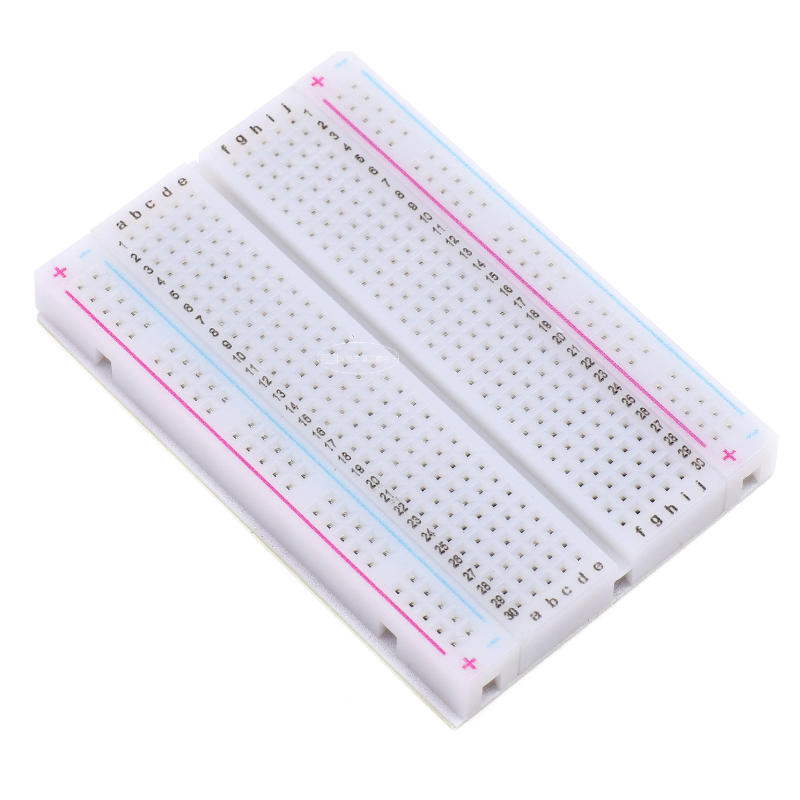
\includegraphics[width=3cm, height=4cm]{Imagenes/proto1.jpg}
	\captionof{figure}{Protoboard}
\end{center}
\subsection{Recistor.}
Un resistor, o resistencia eléctrica, es un componente pasivo fundamental en electrónica que se utiliza para limitar el flujo de corriente eléctrica en un circuito. Su función principal es ofrecer una resistencia al paso de la electricidad, lo que genera una caída de tensión a través de él según la Ley de Ohm. Los resistores están diseñados con un valor específico de resistencia, que se mide en ohmios ($\Omega$), y se fabrican en una variedad de tamaños y potencias para adaptarse a diversas aplicaciones electrónicas. Estos componentes son ampliamente utilizados para ajustar la corriente, dividir el voltaje, proteger componentes sensibles y realizar otras funciones esenciales en la electrónica y la electricidad.
\begin{center}
	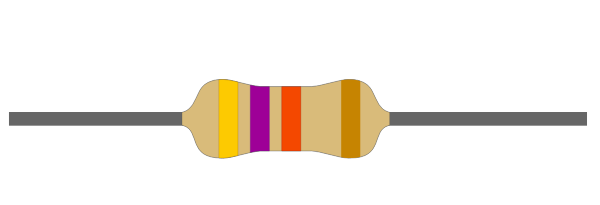
\includegraphics[width=5cm, height=3cm]{Imagenes/resistor.png}
	\captionof{figure}{Recistor}
\end{center}
\subsection{Ley de Ohm.}
La Ley de Ohm es un principio fundamental en la electrónica y la electricidad que establece la relación entre la corriente eléctrica (I), la tensión o voltaje (V) y la resistencia eléctrica (R) en un circuito eléctrico. Fue formulada por el físico alemán Georg Simon Ohm en el siglo XIX y se expresa mediante la siguiente ecuación:
\begin{center}
	$ V=I*R$,  $I=\frac{V}{R}$, $R=\frac{V}{I}$
\end{center}


\subsection{Divisores de corriente y voltaje.}
Los divisores de corriente y voltaje son conceptos fundamentales en la teoría de circuitos eléctricos que se utilizan para analizar y calcular las corrientes y tensiones en diferentes partes de un circuito. Estos divisores son útiles en la resolución de circuitos en serie y en paralelo.
\subsubsection{Divisor de Tensión (Divisor de Voltaje):}
El divisor de tensión se utiliza para calcular la tensión (voltaje) en un punto específico de un circuito en serie. Se basa en la Ley de Ohm y se expresa mediante la siguiente fórmula: 
\begin{center}
$V_{k}=\frac{V_{fc}*R_{k}}{R_{eq}}$
\end{center}
\subsubsection{Divisor de Corriente:}
El divisor de corriente se utiliza para calcular la corriente en una rama específica de un circuito en paralelo. También se basa en la Ley de Ohm y se expresa mediante la siguiente fórmula:
\begin{center}
	$I_{k}=\frac{I_{fc}*R_{eq}}{R_{k}}$
\end{center}
\end{multicols}

\begin{center}
	\begin{adjustbox}{width=540pt}
		\begin{tabular}{|c|c|c|c|c|c|c|c|c|c|c|c|c|c|}
			\hline
			
			 &  & \multicolumn{3}{ |c| }{Teoria} & \multicolumn{3}{ |c| }{Simulación Multisim} & \multicolumn{3}{ |c| }{Simulación Pspice} & \multicolumn{3}{ |c| }{Mediciones en laboratorio} \\
			\hline
			 & Valor de resistores en ohms & \multicolumn{3}{ |c| }{$R_{eq} = 2.108k\Omega$}  & \multicolumn{3}{ |c| }{$R_{eq} = 2.109k\Omega$} & \multicolumn{3}{ |c| }{$R_{eq}=2.1188K\Omega$} & \multicolumn{3}{ |c| }{$R_{eq} = 2.089k\Omega$} \\
			\hline
			 &  & Tensión & Corriente & Potencia & Tensión & Corriente & Potencia & Tensión & Corriente & Potencia & Tensión & Corriente & Potencia \\ 
			\hline
			$R_{1}$ & 680 & 2.9V & 4.26mA & 12.3mW & 2.092V & 4.268mA & 12.386mW & 2.9310V & 4.2478mA & 12.450mW & 2.8V & 4.20mA & 11.76mW  \\
			\hline
			$R_{2}$ & 560 & 2.39V & 4.26mA & 10.1mW & 2.39V & 4.268mA & 10.201mW & 2.3788V & 4.2478mA & 10.105mW & 2.35V & 4.27mA & 10.03mW   \\
			\hline
			$R_{3}$ & 470 & 2.00V & 4.26mA & 8.52mW & 2.006V & 4.268mA & 8.561mW & 1.9965V & 4.2478mA & 8.4805mW & 1.98V & 4.29mA & 8.49mW  \\
			\hline
			$R_{4}$ & 330 & 1.40V & 4.26mA & 5.96mW & 11.480V & 4.268mA & 6.011mW & 1.4018V & 4.2478mA & 5.9544mW & 1.39V & 4.29mA & 5.96mW \\
			\hline
			$R_{5}$ & 220 & 0.29V & 1.31mA & 0.37mW & 0.029V & 1.334mA & 391.343$\mu W$ & 292.035V & 2.9204mA & 852.847 $\mu W$ & 0.28V & 1.31mA & 0.36mW   \\
			\hline
			$R_{6}$ & 100 & 0.02V & 2.90mA & 0.058mW & 0.029V & 2.934mA & 860.955$\mu W$ & 292.035V & 1.3274mA & 387.658$\mu W$ & 0.28V & 2.93mA & 0.082mW   \\
			\hline
		\end{tabular}
	\end{adjustbox}
\end{center}
\begin{multicols}{2}

\section{Primera etapa. Teoría}
\begin{center}
	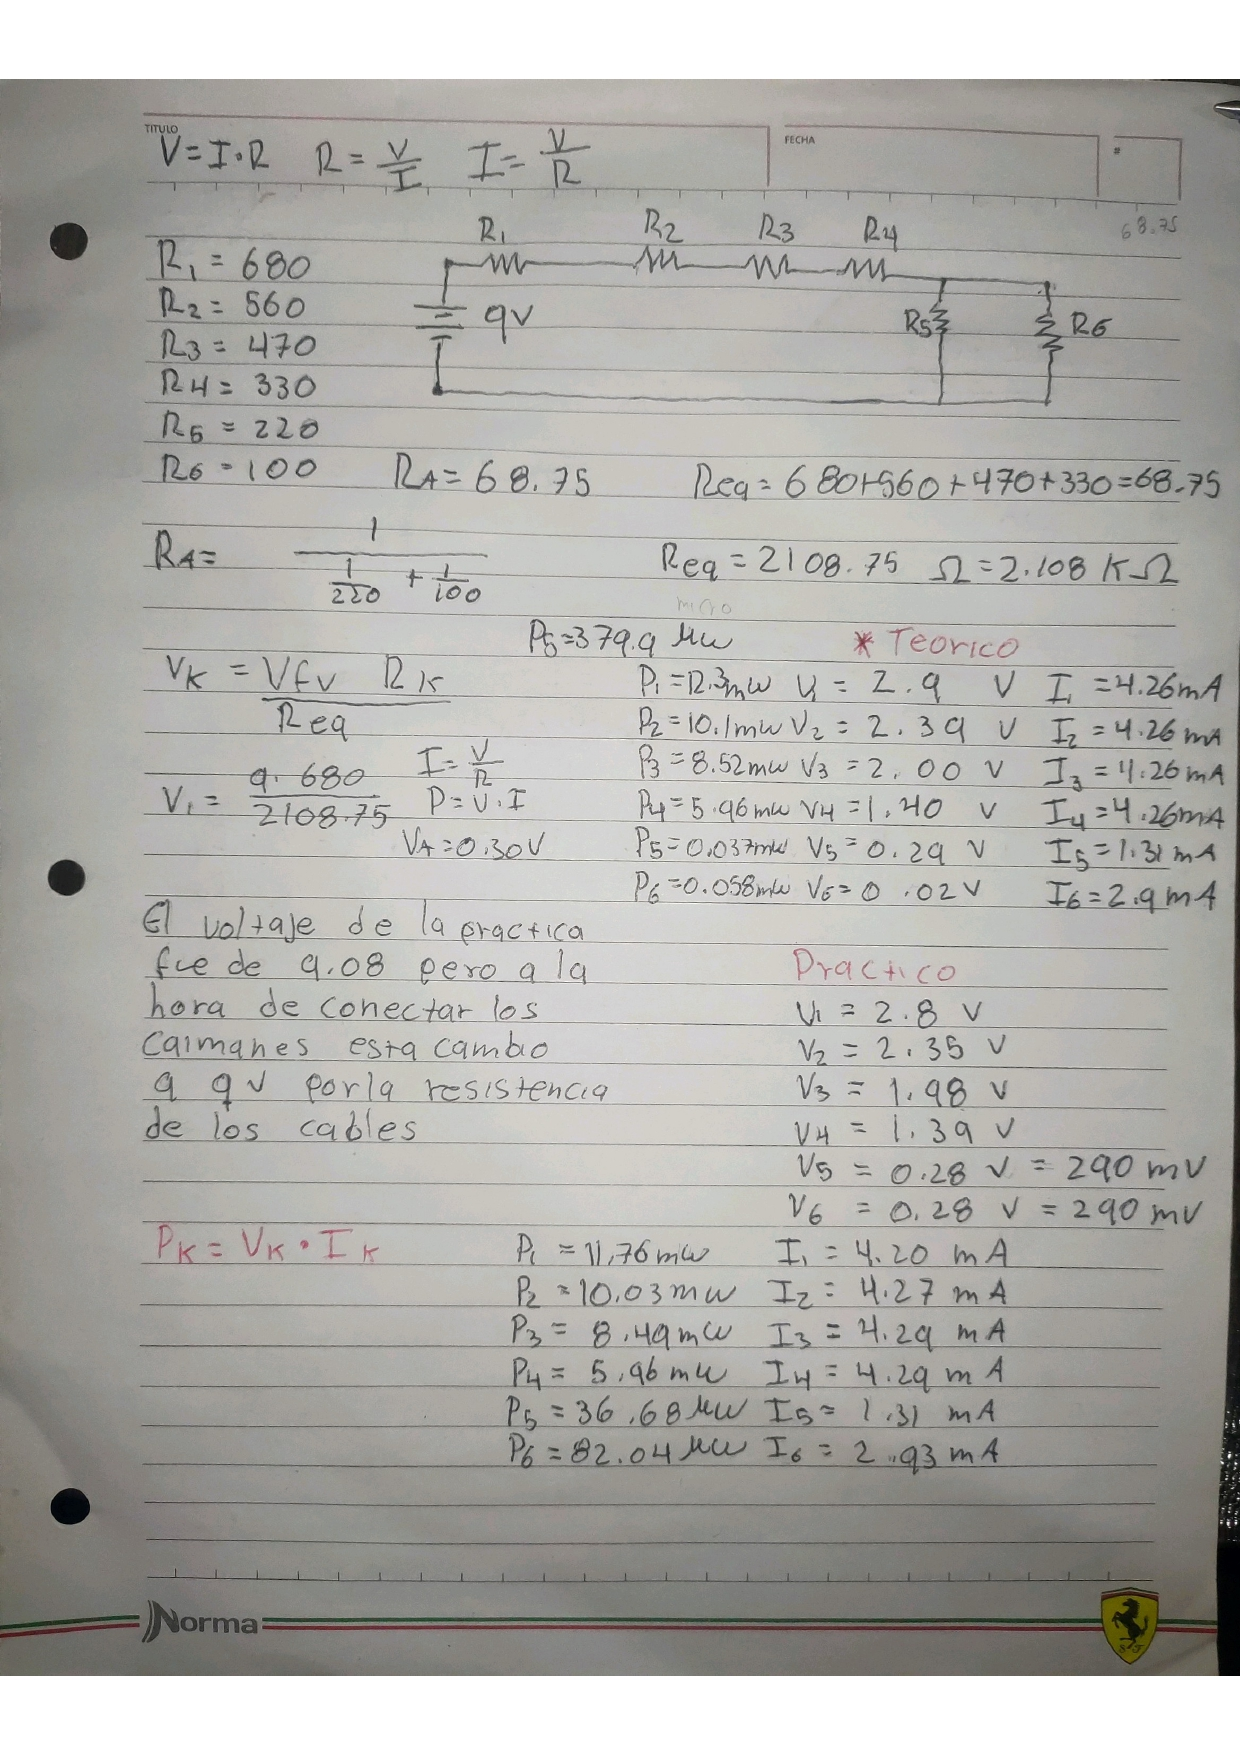
\includegraphics[width=5cm, height=7.5cm]{Imagenes/notas.jpg}
	\captionof{figure}{Recopilacion de los calculos}
	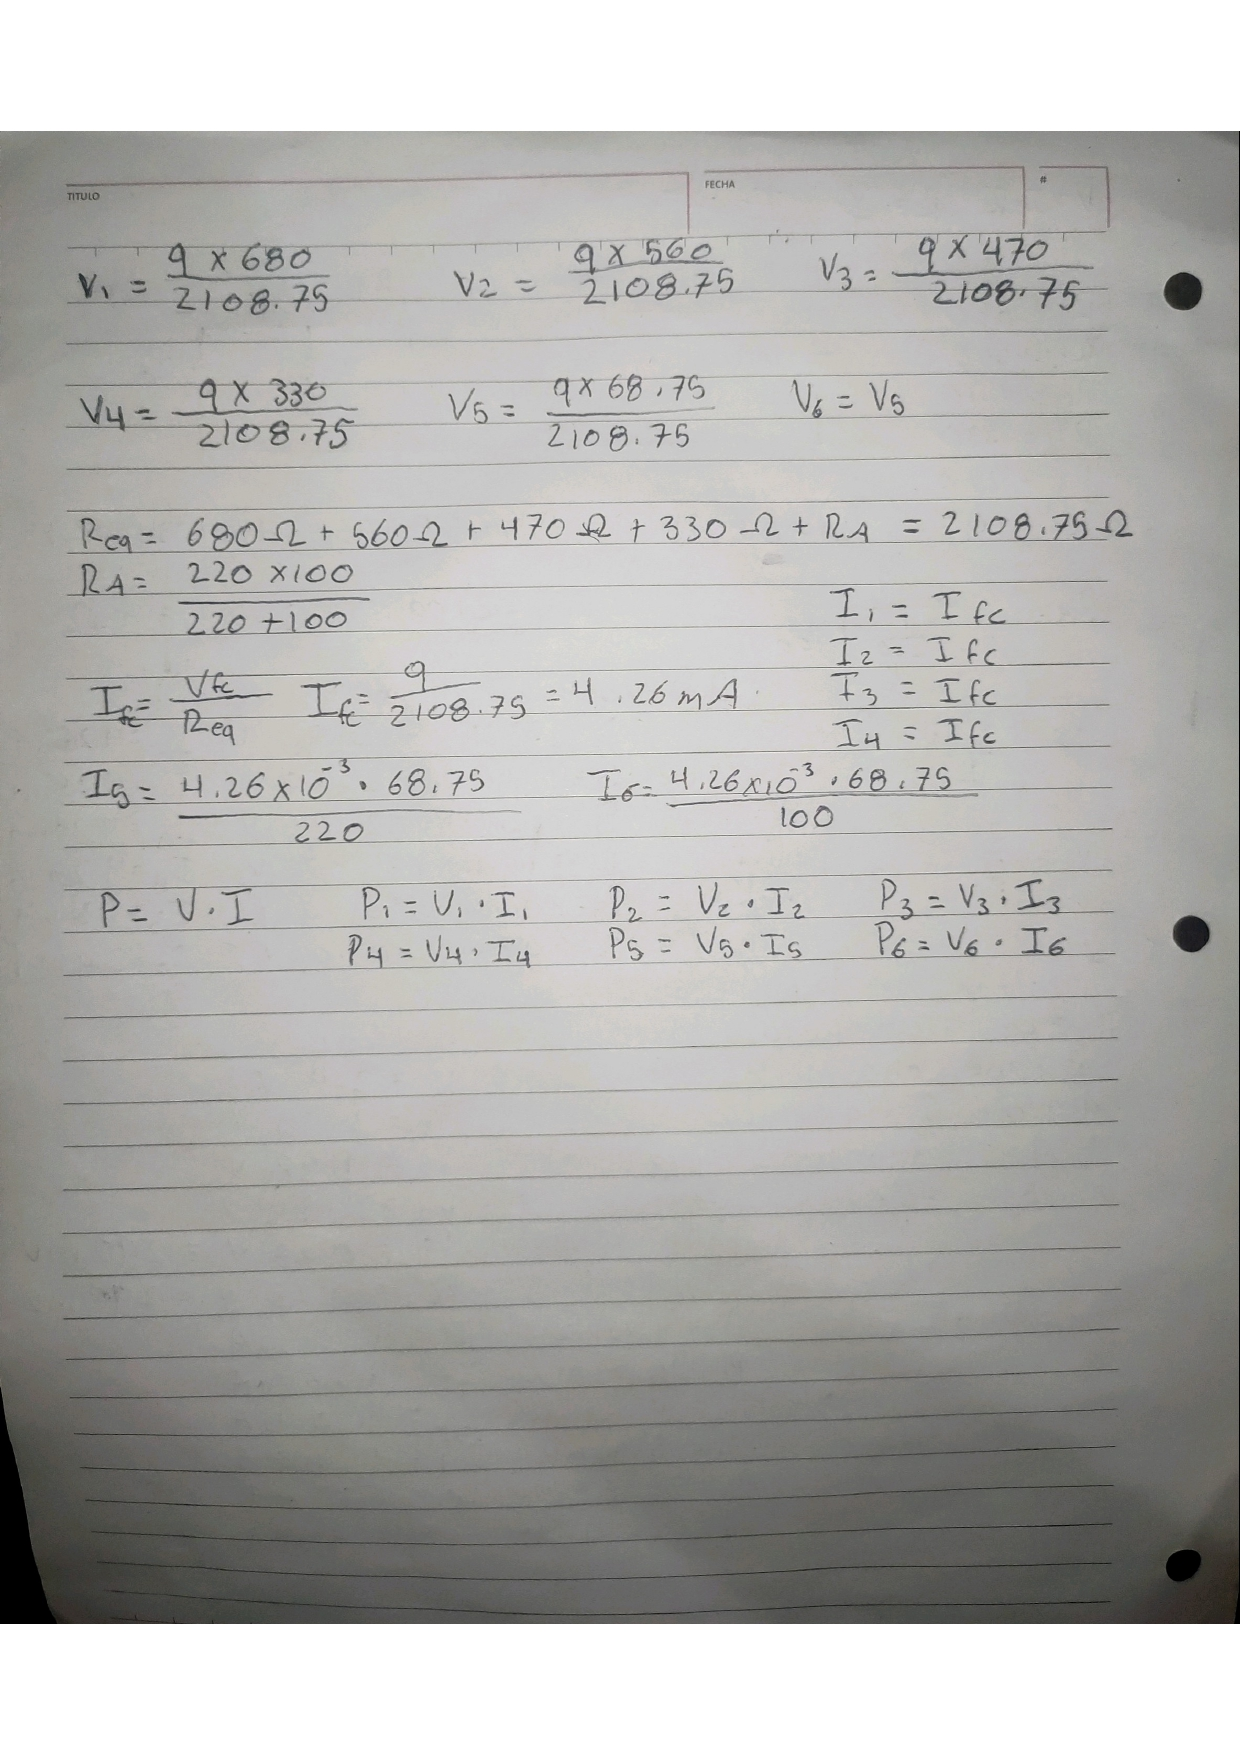
\includegraphics[width=5cm, height=8cm]{Imagenes/cal.jpg}
	\captionof{figure}{Calculos en la teoria}
\end{center}
\section{Segunda etapa. Simulación}
\subsection{Utilizando el programa de simulación Multisim.}
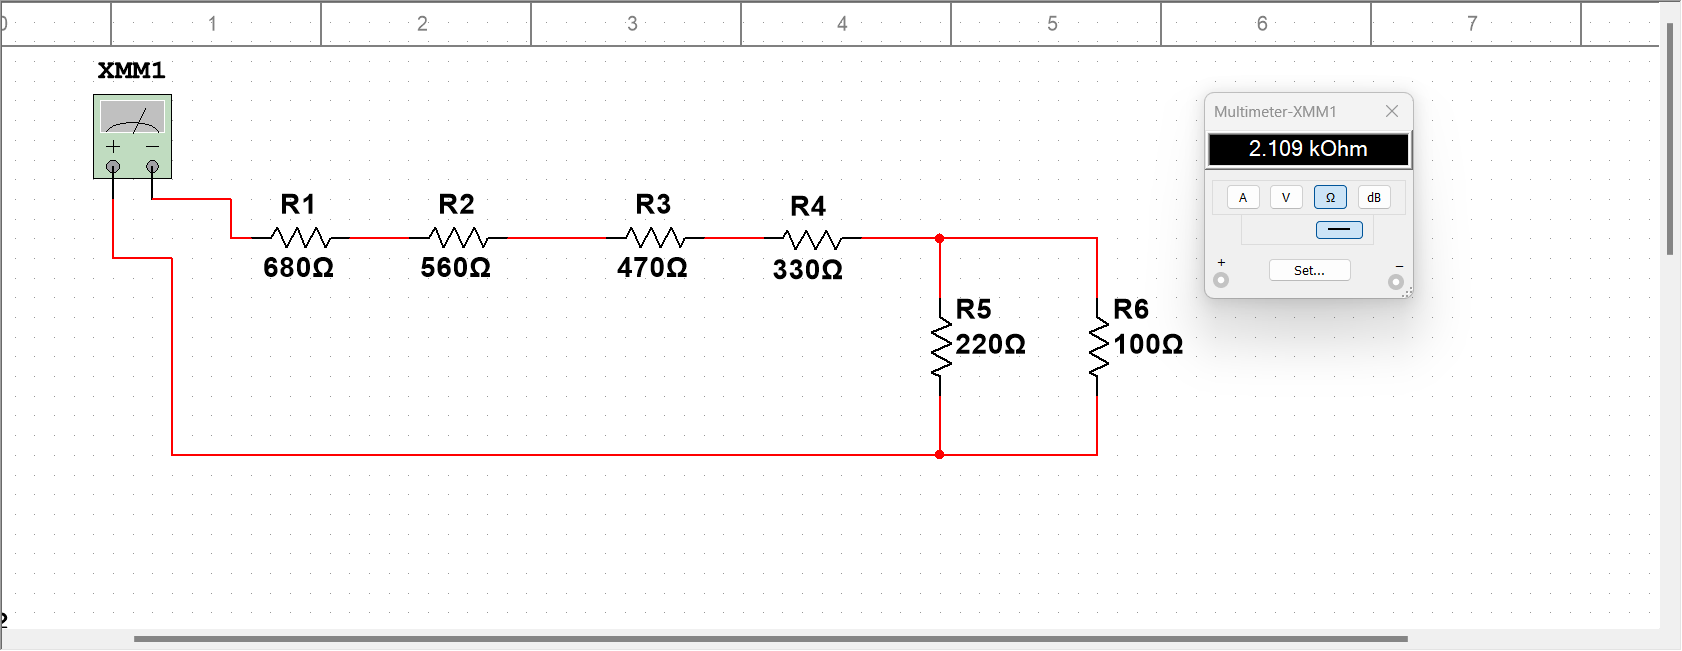
\includegraphics[width=\linewidth]{Imagenes/recistencia eq.png}
\captionof{figure}{Recistencia equivalente del circuito}
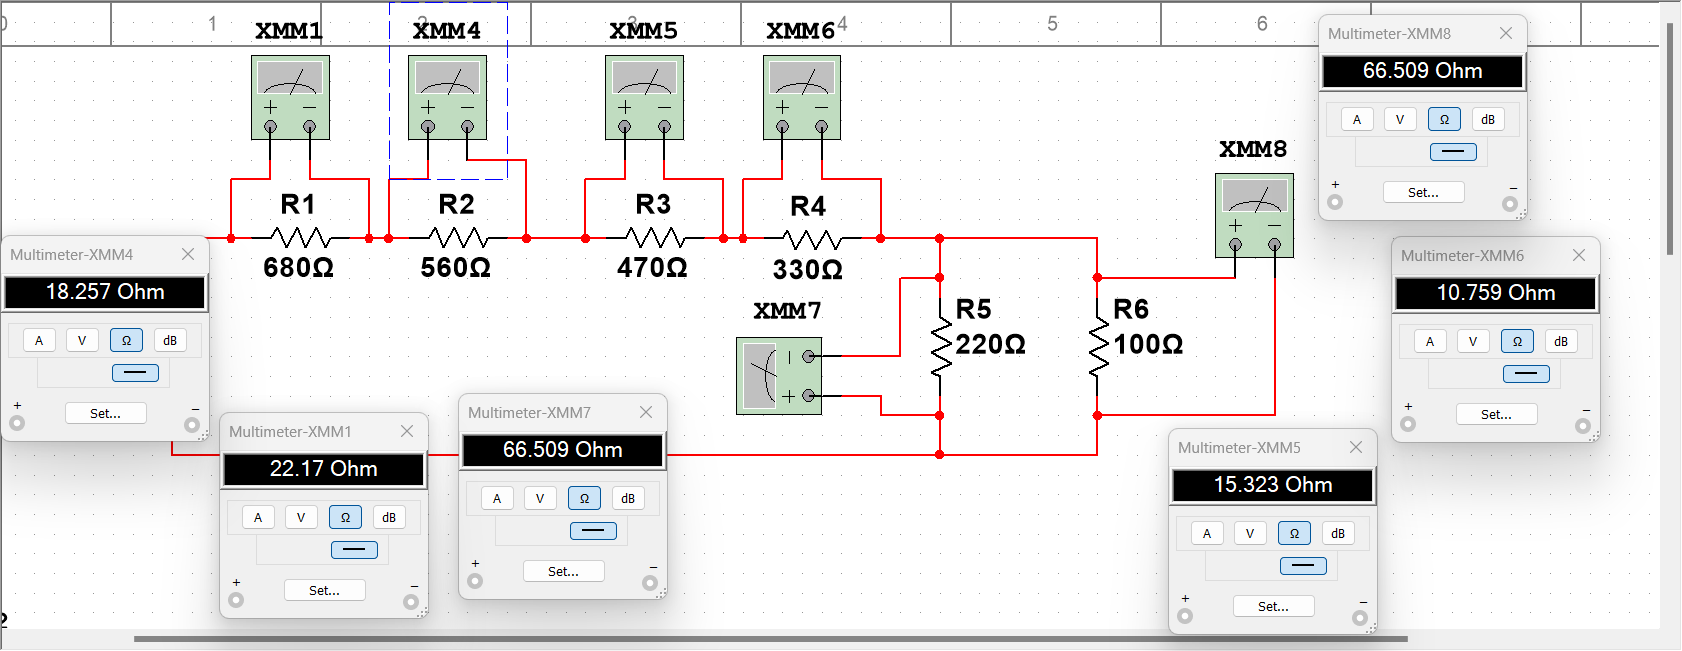
\includegraphics[width=\linewidth]{Imagenes/recistencias k.png}
\captionof{figure}{Valor de cada recistencia en el circuito}
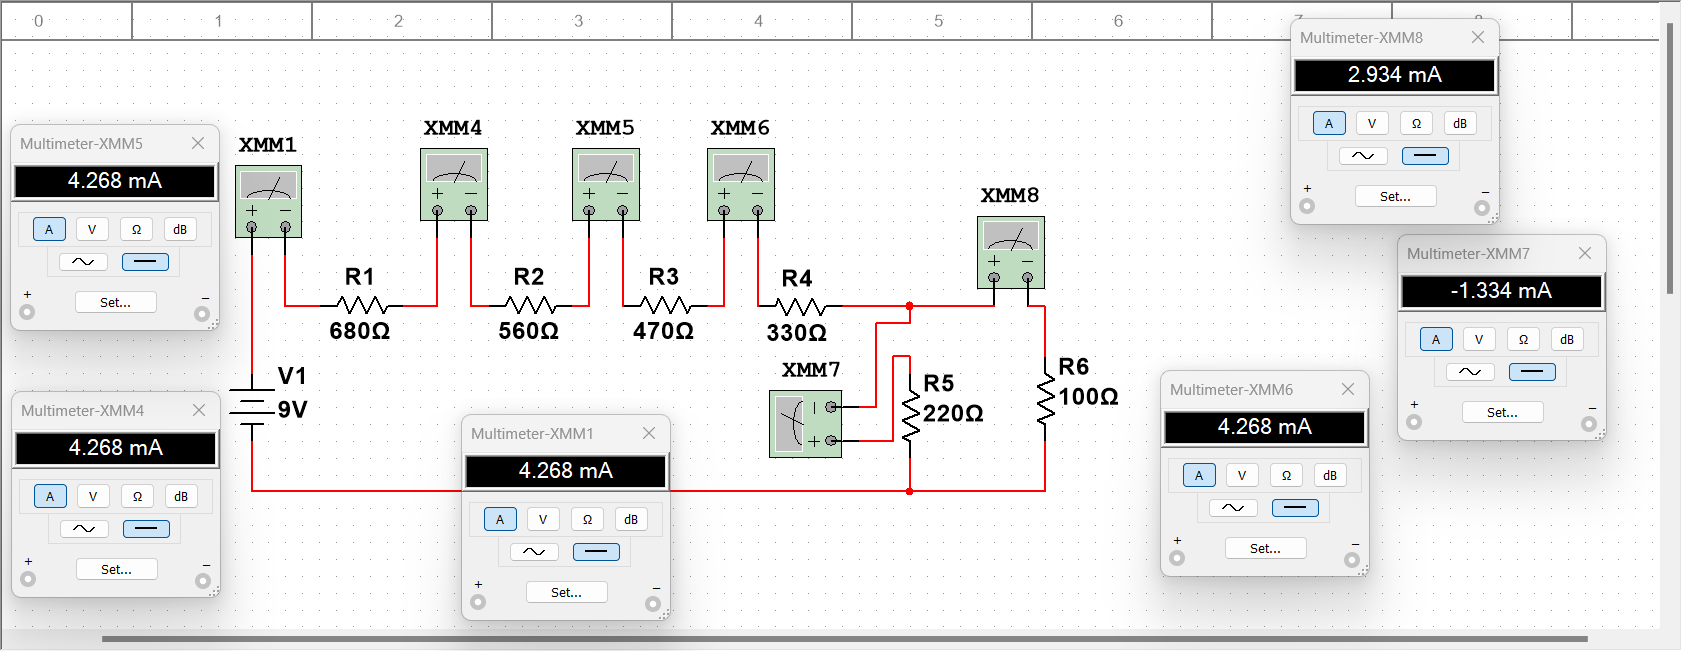
\includegraphics[width=\linewidth]{Imagenes/corriente k.png}
\captionof{figure}{Valor de cada corriente en el circuito}
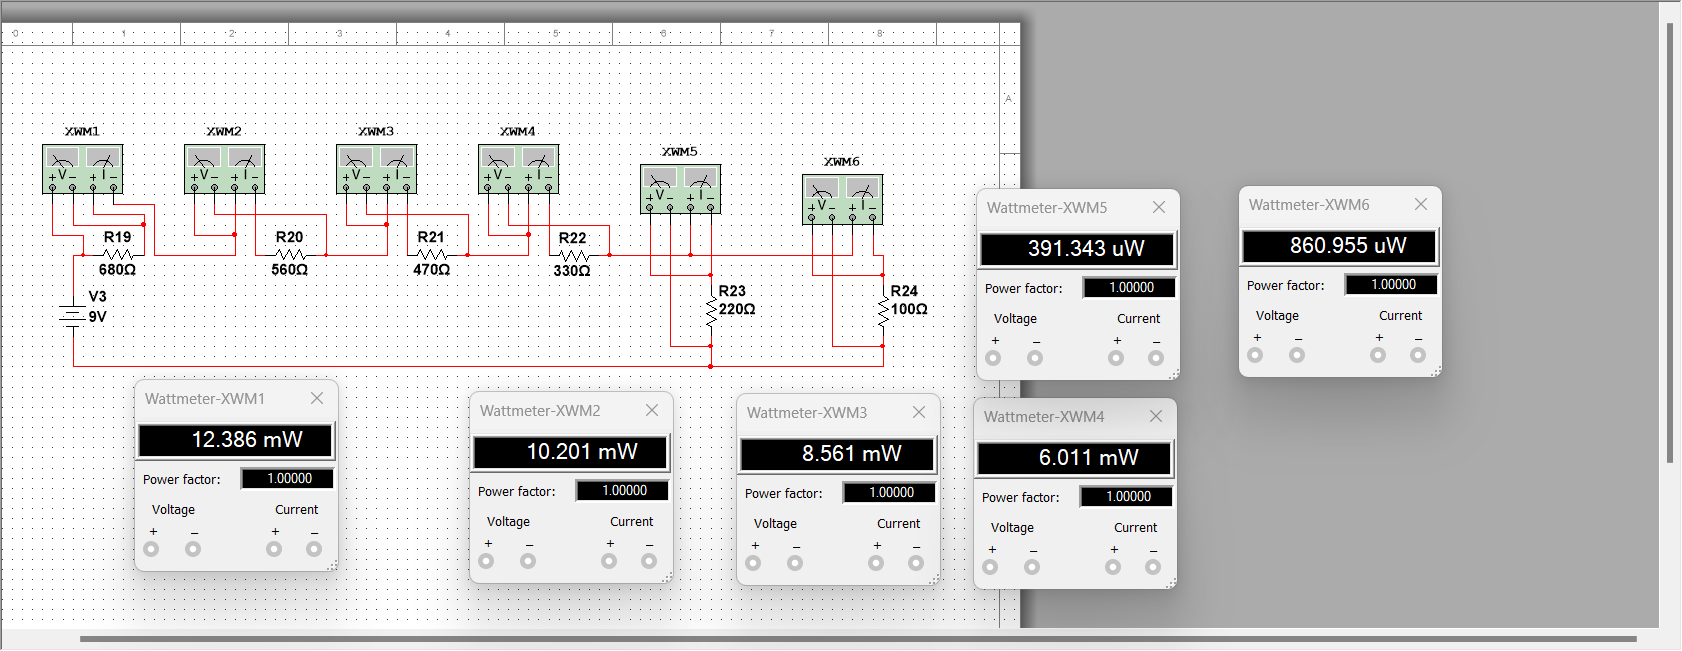
\includegraphics[width=\linewidth]{Imagenes/potencias.png}
\captionof{figure}{Valor de la potencia de cada componente}
\subsection{Ahora Utilizando el programa de Pspice:}
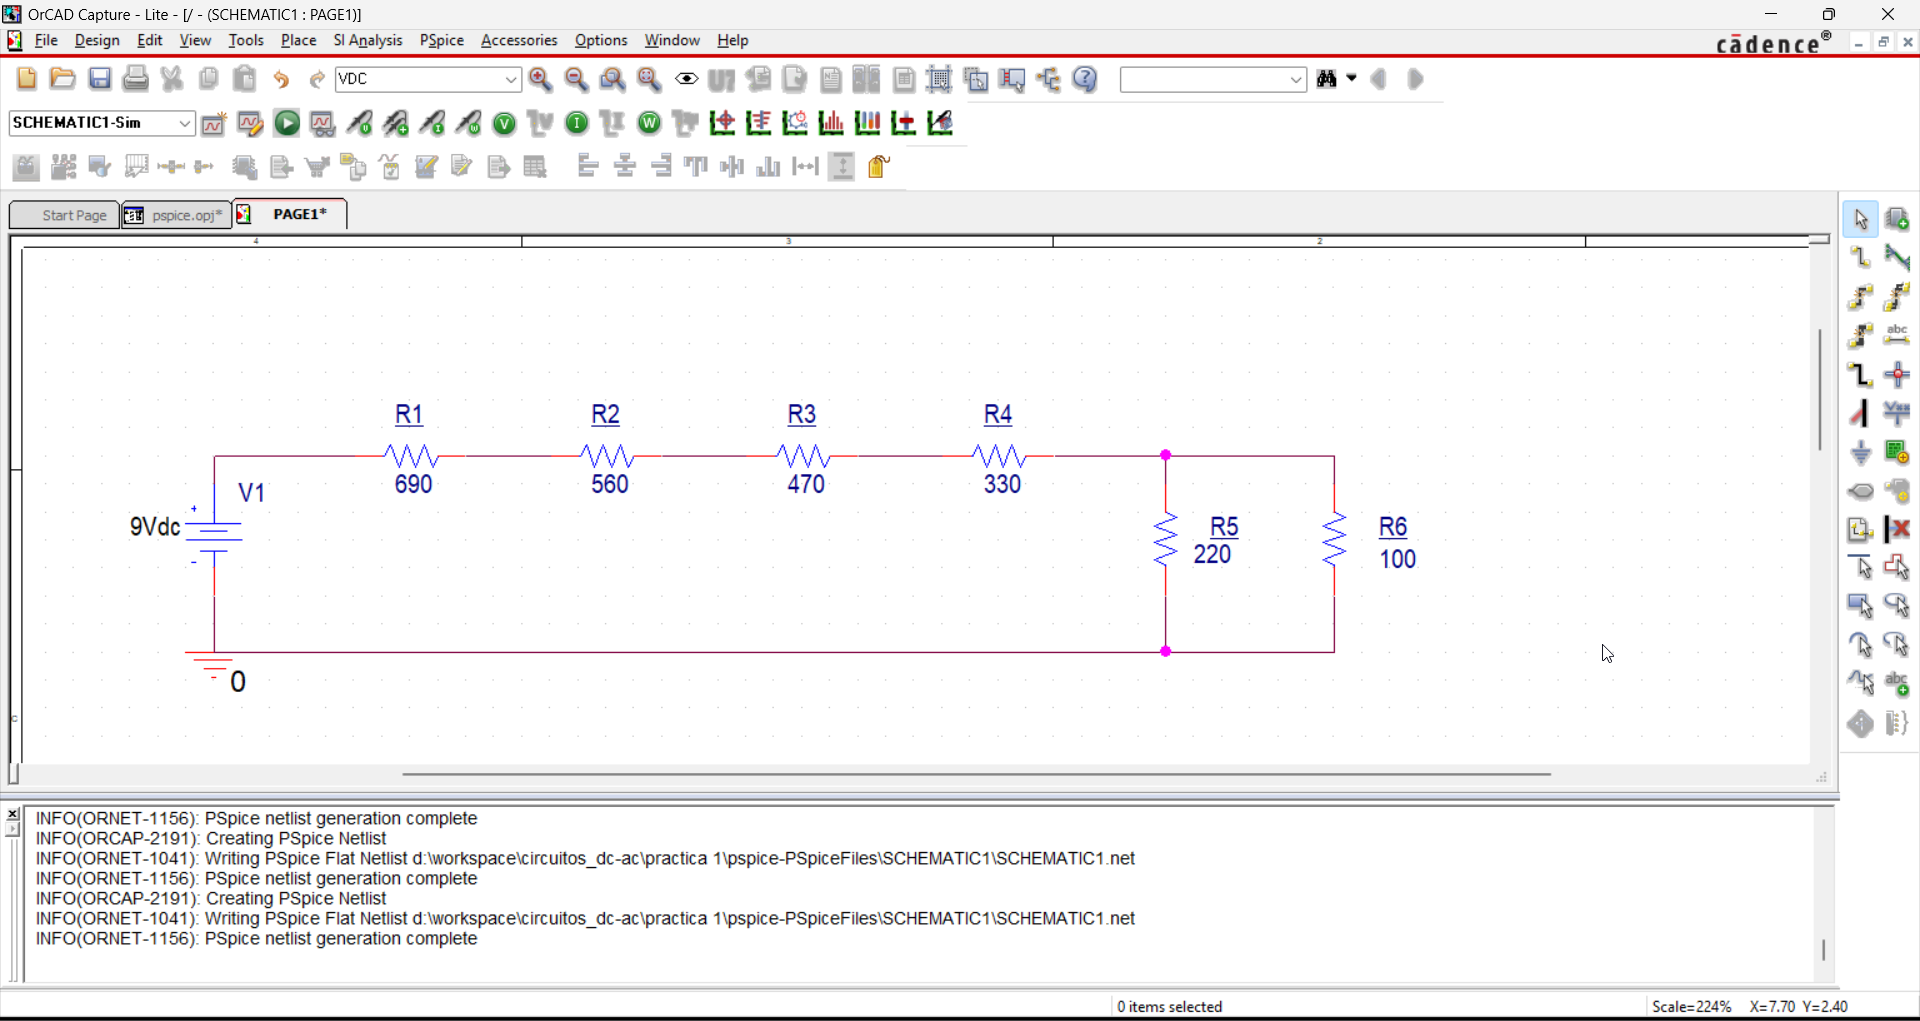
\includegraphics[width=\linewidth]{Imagenes/psipce.png}
\captionof{figure}{Circuito simulado en Pspice} 
Para poder calcular la recistencia equivalente en este programa utilizamos la ley de ohm exactamente $R=frac_{V}{I}$ graficando esta formula tenemos lo siguiente: 
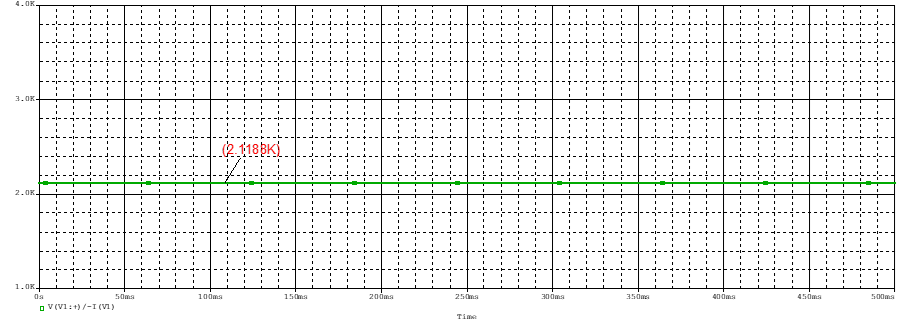
\includegraphics[width=\linewidth]{Imagenes/reseq.png}
\captionof{figure}{Grafica de la recistencia equivalente}

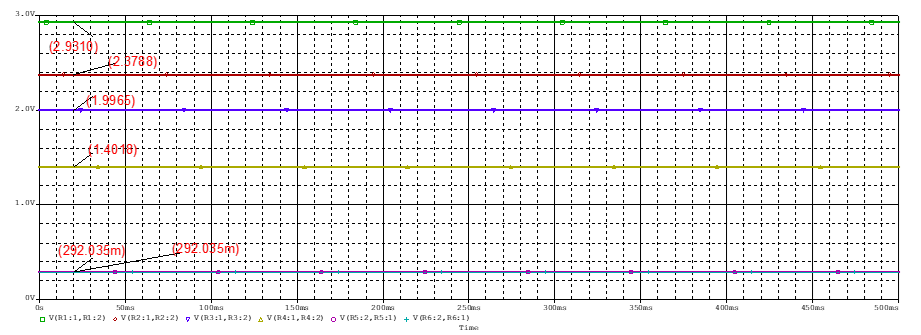
\includegraphics[width=\linewidth]{Imagenes/vk.png}
\captionof{figure}{Grafica del tensión de cada recistor}
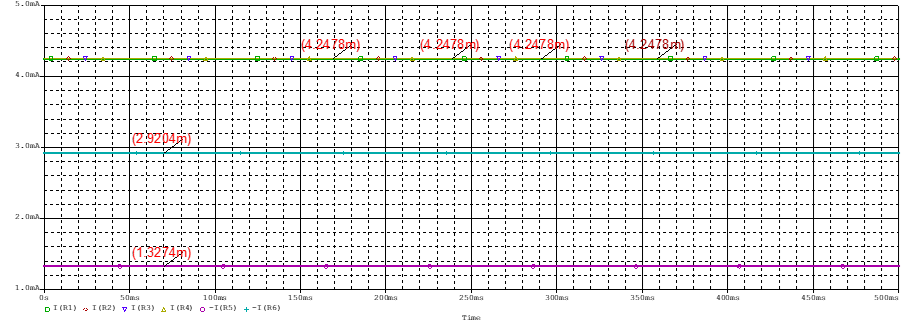
\includegraphics[width=\linewidth]{Imagenes/intensidad.png}
\captionof{figure}{Grafica de la corriente de cada elemento}
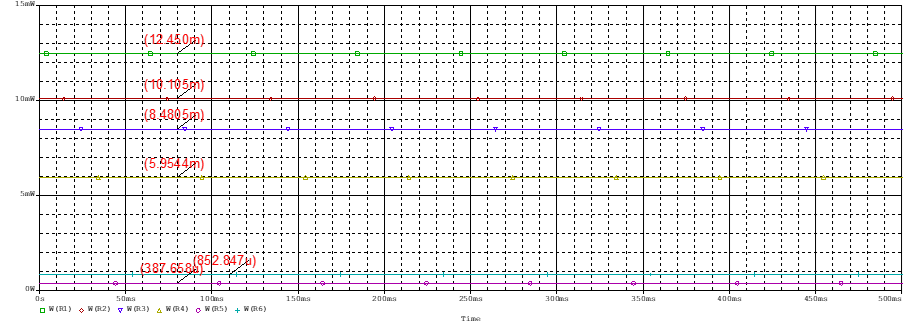
\includegraphics[width=\linewidth]{Imagenes/potenciak.png}
\captionof{figure}{Grafica de la potencia en cada recistor}

\section{Tercera etapa. Mediciones con instrumentos en laboratorio}
Por falta de imagenes tomadas en el laboratorio se muestran imagenes tomadas la casa del alumno tomando la medicion de la recitencia equivalente con su multimetro propio 
\begin{center}
	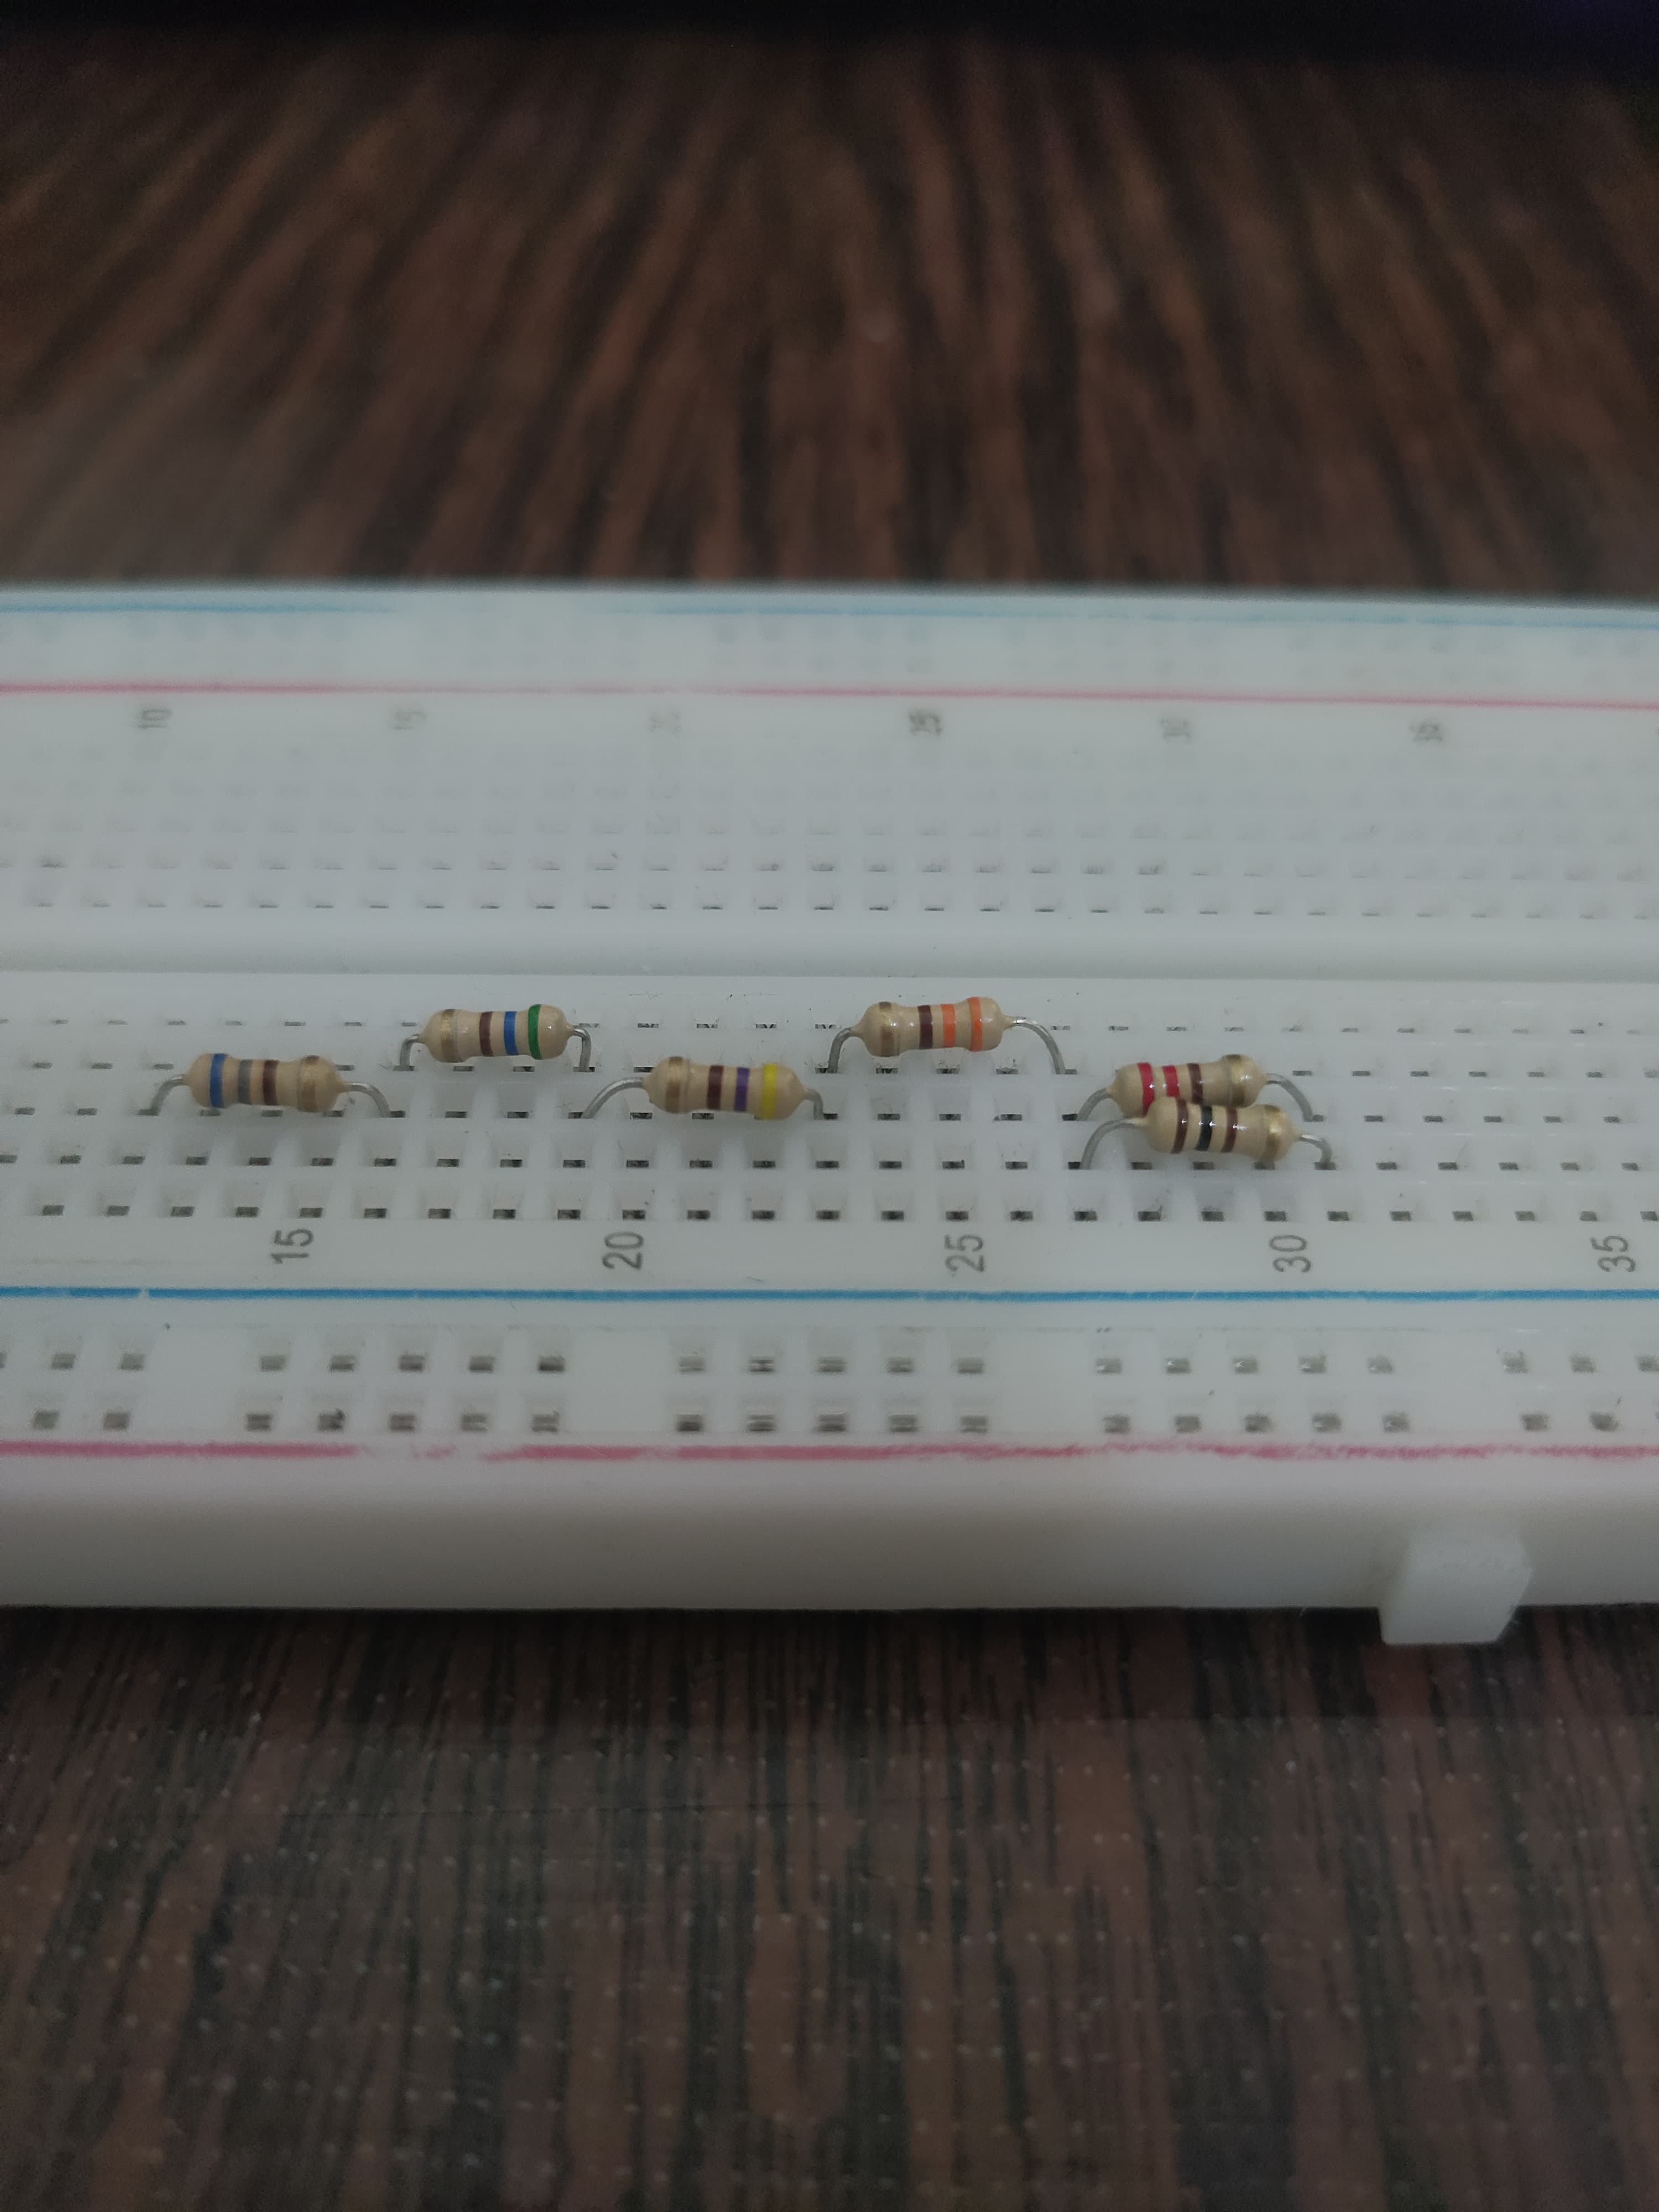
\includegraphics[width=4cm, height=6cm]{Imagenes/Proto.jpeg}
	\captionof{figure}{Circuito armado en la protoboard}
	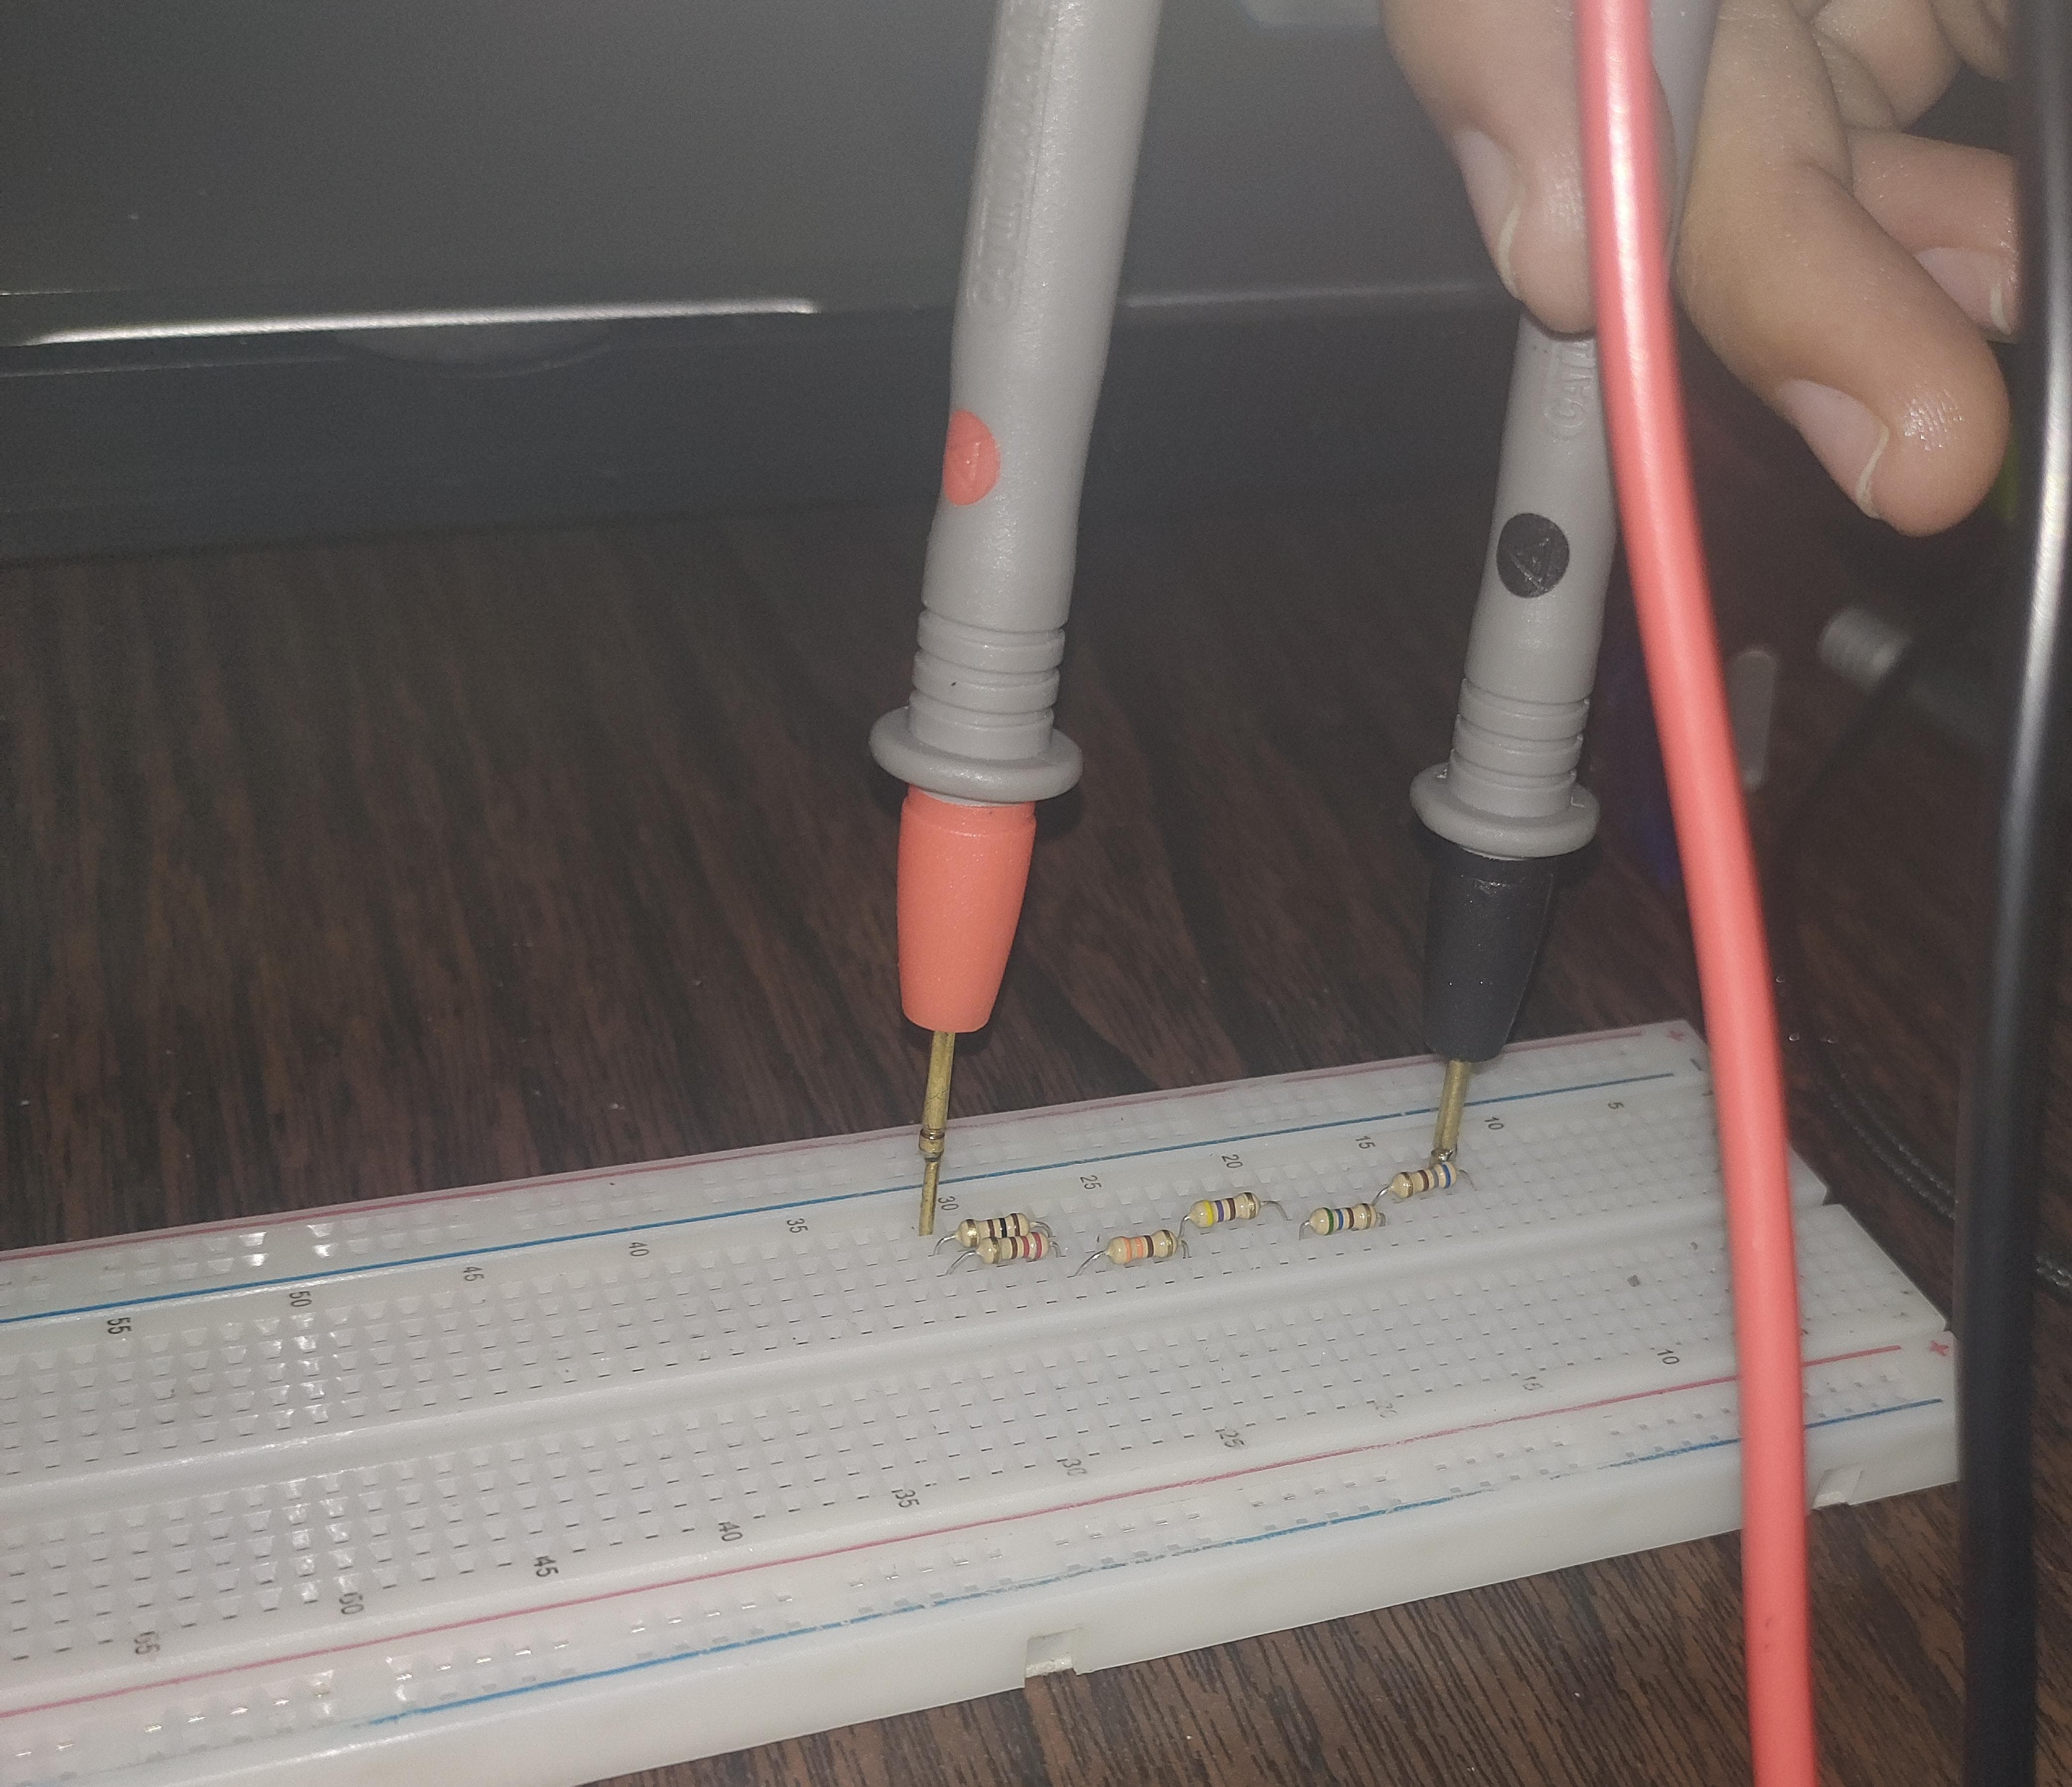
\includegraphics[width=4cm, height=6cm]{Imagenes/mediciones.jpeg}
	\captionof{figure}{Medicion de la recistencia equivalente}
	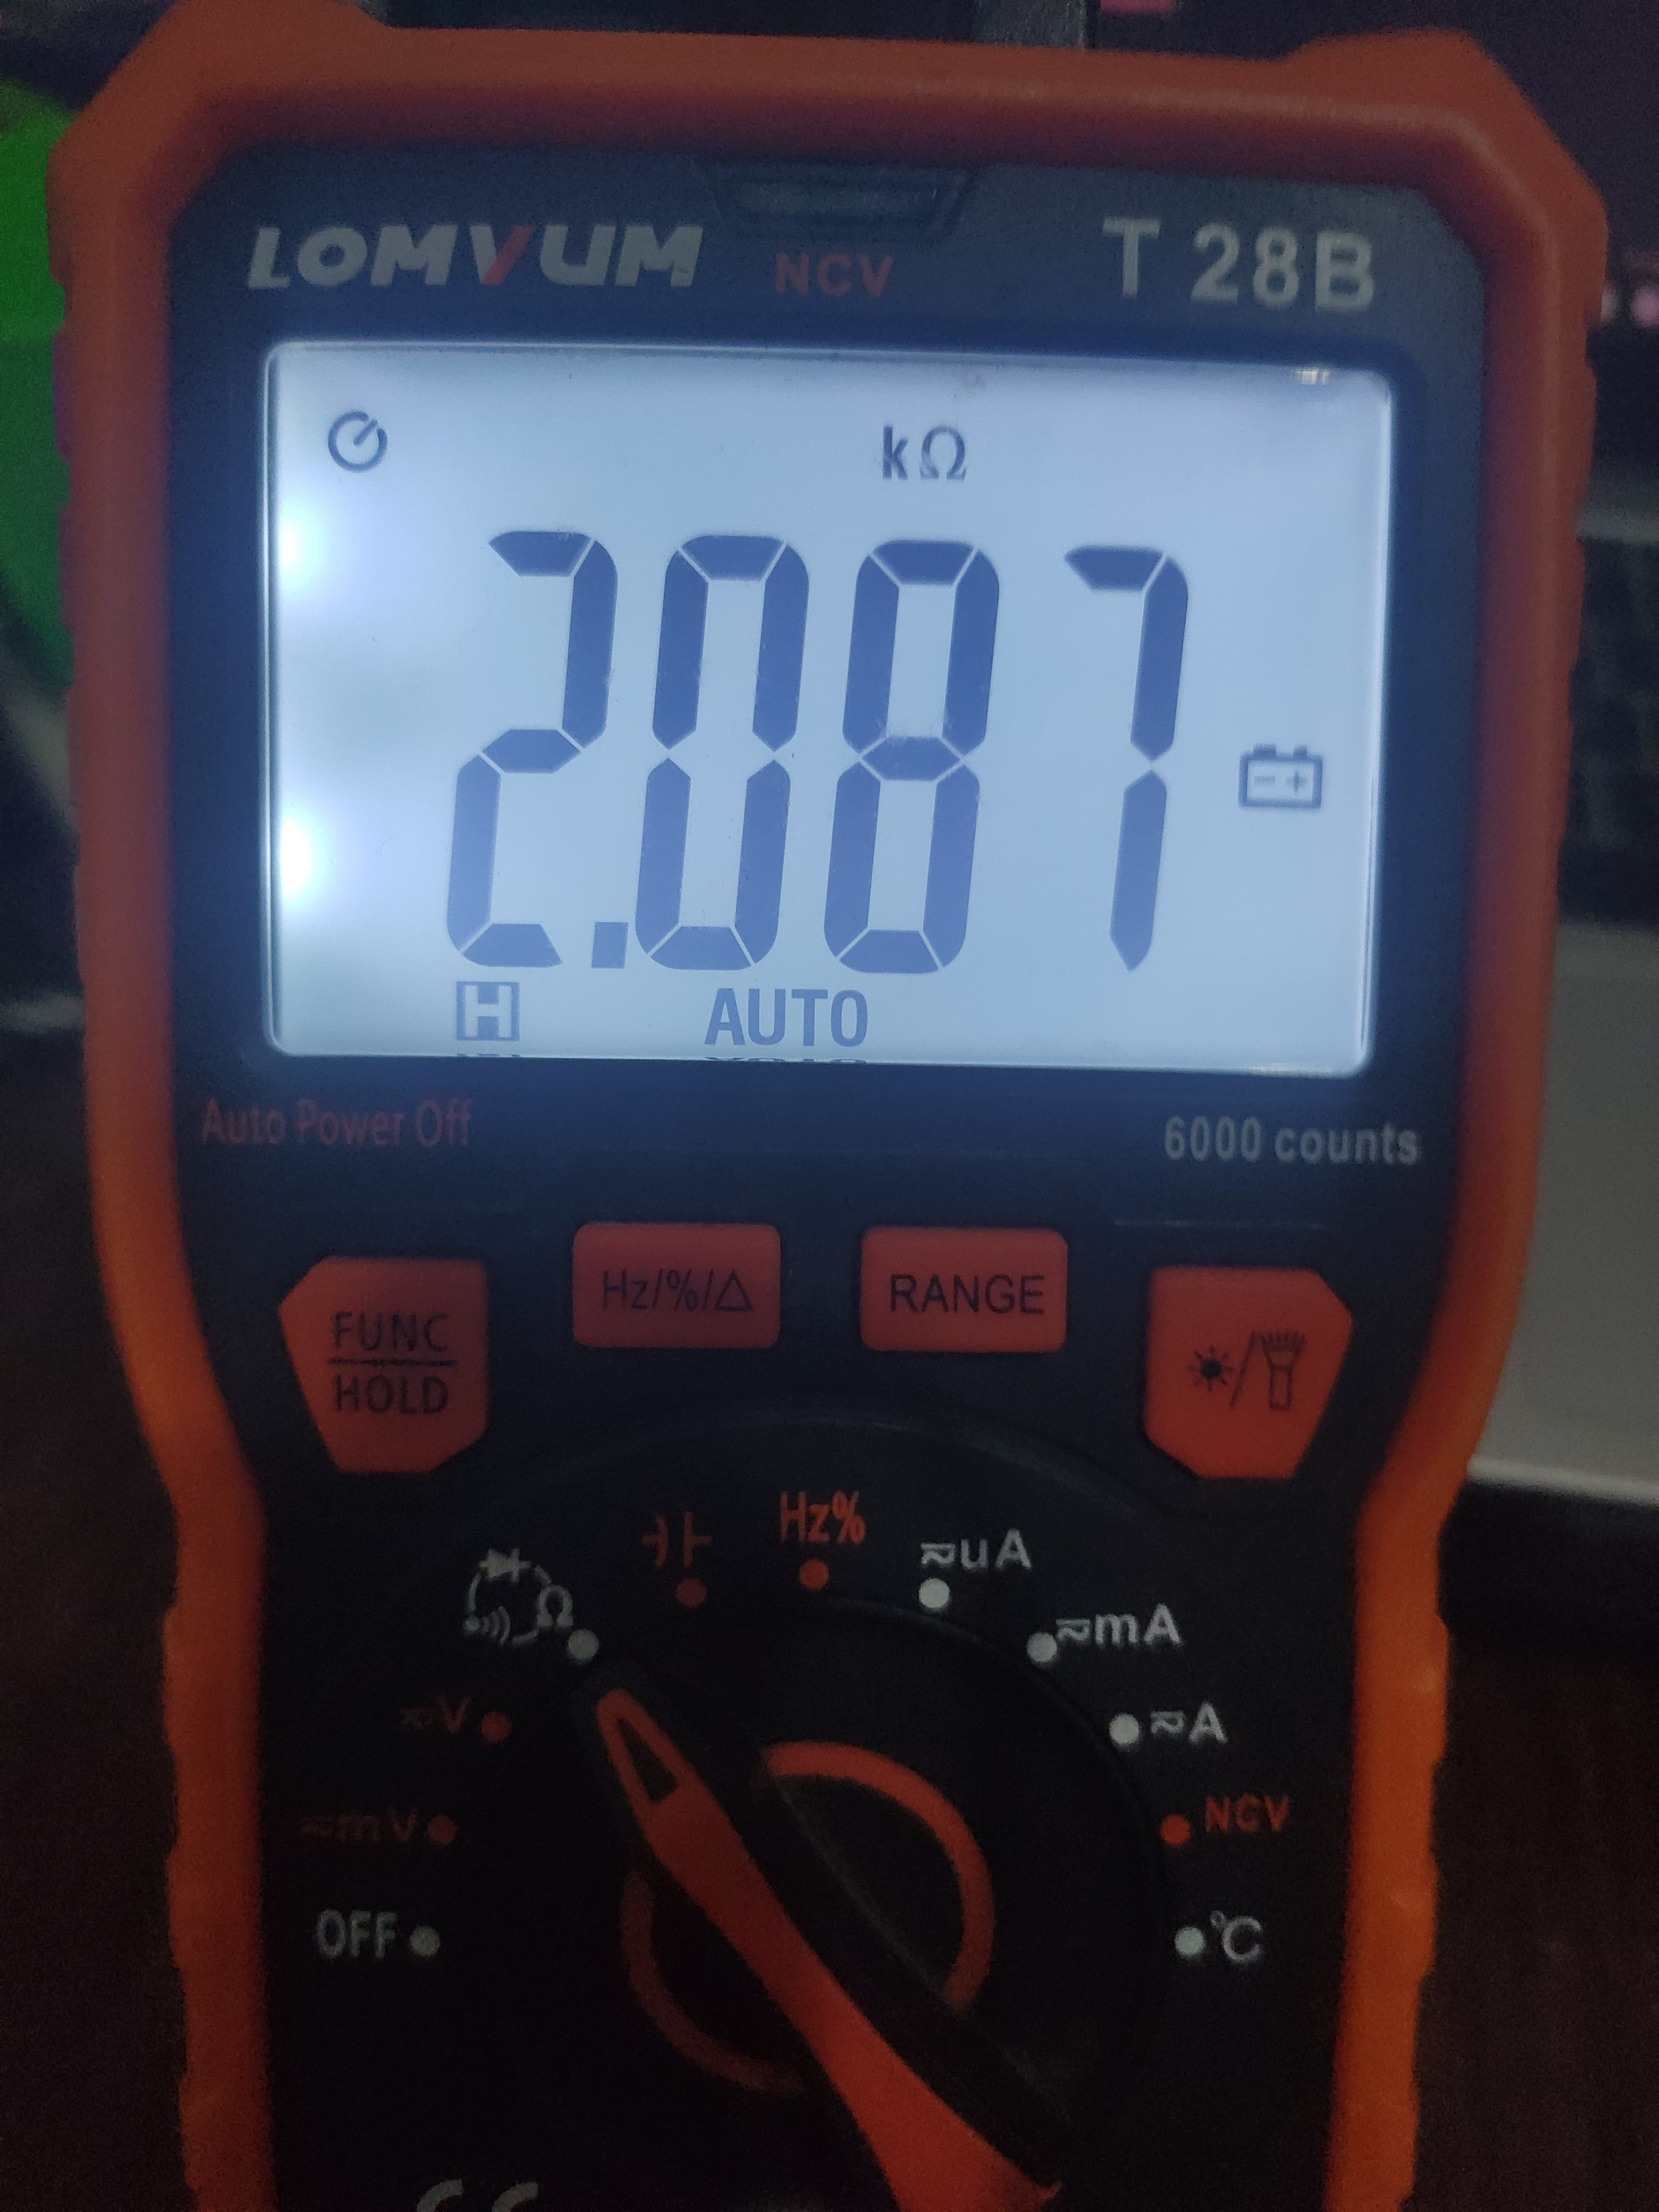
\includegraphics[width=4cm, height=6cm]{Imagenes/muldata.jpeg}
	\captionof{figure}{Resultados de la medicion}
\end{center}


\end{multicols}

\end{document}
